\documentclass[12pt,a4paper]{scrartcl}
\usepackage{url, pdflscape}
\usepackage[final]{pdfpages}
\usepackage[colorlinks]{hyperref}
\usepackage{longtable}
\title{Student Robotics Risk Assessment Form}

\begin{document}
\maketitle

\begin{description}
\item[Activity being assessed:] Student Robotics Kickstart
\item[Persons at risk:] Competitors, Team Leaders, Blueshirts
\item[Location:] Multiple Locations
\end{description}

\begin{description}
\item[Assessor's name:] Andrew Busse
\item[Responsible Persons:] Sam Phippen (SC - Events); Rich Barlow (SC -
Engineering); 
\item[Date of assessment:] \date{\today}
\end{description}
\clearpage

\newcommand{\risk}[4]{
 #1 & #2 & #3 & #4 \\
}

\begin{landscape}
\section{Risks}
The following risks have been considered for the Student Robotics Kickstart event. 
Further description of the meaning of risk ratings (presented in this section as
$L \times S$) can be found in the next section.

As this activity is being run at multiple locations, local events will release an appendix to
this assessment containing additional risks and control measures, and the building / area risk
assessments. The event coordinator will also carry out a Point of Work Risk Assessment on the
morning of the event, defining any additional risks that present themselves.


\centering
\begin{longtable}{|p{17em}|p{8cm}|p{4cm}|p{4em}|}
\hline
\textbf{Hazard} & \textbf{Control Measures} & \textbf{Responsible Person} & \textbf{Risk Rating} \\
\hline
\endhead

\endfoot

\risk{Injury while using manual tools (Screwdrivers, Wire Snippers)}
{Student Robotics Blueshirts will supervise all use of tools and materials in the
hacking sessions}
{SC - Events}
{1}
\hline

\risk{Interaction with robots: electric shock, minor injury}
{No exposed voltages above ELV (120V DC, 50V AC) present on any boards, no
stored energy above 5J (save the batteries -- see below)}
{SC - Engineering}
{2}

\risk{}
{All electronic boards undergo a full system check before delivery, and are
delivered in suitably robust cases designed to contain component failures}
{SC - Engineering}
{}

\risk{}
{Documentation related to kit usage (at \url{https://www.studentrobotics.org/docs})
must be clear, up to date, and reviewed once per year}
{SC - Engineering}
{}

\risk{}
{Boards must remain in their cases.}
{Team Leader}
{}

\risk{}
{Wiring to be inspected by SQEP before robots switched on: Polarities are correct, no
exposed / frayed wire strands, colour coding is respected, wiring is kept tidy}
{SC - Engineering, SC - Events}
{}

\hline
\risk{Trip Hazard from trailing extension leads}
{Extension leads taped down and inspected regularly, kept away from walkways
where reasonably practicable}
{SC - Events}
{1}

\hline
\risk{Misuse of batteries}
{Charging to be performed in the exact manner described in
\url{https://www.studentrobotics.org/docs/kit/batteries}. This will be done
under direct supervision of SQEP}
{SC - Engineering, SC - Events}
{4}

\risk{}
{Chargers and batteries tested, charging bags inspected before being delivered
to teams}
{SC - Engineering}
{}

\risk{}
{Documentation related to battery usage (at the above link) must be clear, up to date,
and reviewed once per year}
{SC - Engineering}
{}

\risk{}
{SQEP Blueshirts to quickly and safely dispose of any battery displaying signs of
swelling, damage or other abnormality}
{SC - Events, SC - Engineering}
{}

\hline
\risk{Allergies to fibres in Charging Bags}
{Use gloves (any type) to minimise contact between fibres and hand, if persons
are known to be allergic to glass fibres.}
{Team Leader}
{1}
\hline

\end{longtable}
\end{landscape}

\begin{landscape}

\section{Assessment Guidance}

The risk ratings of the risks in the previous section are calculated by multiplying $L$, the likelihood rating, by $S$, the severity rating.

\bigskip
\begin{minipage}[b]{0.5\linewidth}
\begin{tabular}[c]{lc}
\hline
  \textbf{Likelihood} & \textbf{Likelihood rating} \\
\hline
  Very unlikely & 1 \\
  Unlikely & 2 \\
  Likely & 3 \\
  Fairly likely & 4 \\
  Very likely & 5 \\
\hline
\end{tabular}
\end{minipage}
\begin{minipage}[b]{0.5\linewidth}
\begin{tabular}[c]{lc}
\hline
  \textbf{Severity} & \textbf{Severity rating} \\
\hline
  First Aid injury/illness & 1 \\
  Minor injury/illness & 2 \\
  `3 day' injury/illness & 3 \\
  Major injury/illness & 4 \\
  Fatality/disabling injury & 5 \\
\hline
\end{tabular}
\end{minipage}
\bigskip

The following should be used to rate the risk and plan corrective action:
\bigskip
\newcommand{\riskinfo}[4]{
  #1 & #2 & #3 & #4 \\
}

\begin{tabular*}{\linewidth}[c]{cccp{33em}}
\hline
  \textbf{Risk Rating} & \textbf{Category} & \textbf{Tolerability} & \textbf{Comments} \\
\hline

  \riskinfo{1--2}{Very Low}{Acceptable}
  {No further action is necessary other than to ensure that the controls are maintained.}

  \riskinfo{3--4}{Low}{Acceptable}
  {No additional controls are required unless they can be implemented at very low cost (in terms of time, money and effort).}

  \riskinfo{5--7}{Medium}{Tolerable}
  {Consideration should be given as to whether the risks can be lowered, where applicable, to a tolerable level, and preferably acceptable level, but the costs of additional risk reduction measures should be taken into account.  The risk reduction measures should be implemented within a defined time period.}

  \riskinfo{8--14}{High}{Tolerable}
  {Substantial efforts should be made to reduce the risk.  Risk reduction measures should be implemented urgently within a defined time period and it might be necessary to consider suspending or restricting the activity, or to apply interim risk control measures, until this has been completed. Considerable resources might have to be allocated to additional control measures.}

  \riskinfo{15 and above}{Very High}{Unacceptable}
  {Substantial improvements in risk control are necessary, so that risk is reduced to a tolerable or acceptable level.}

\hline
\end{tabular*}

\end{landscape}


%\clearpage

%\newpage
%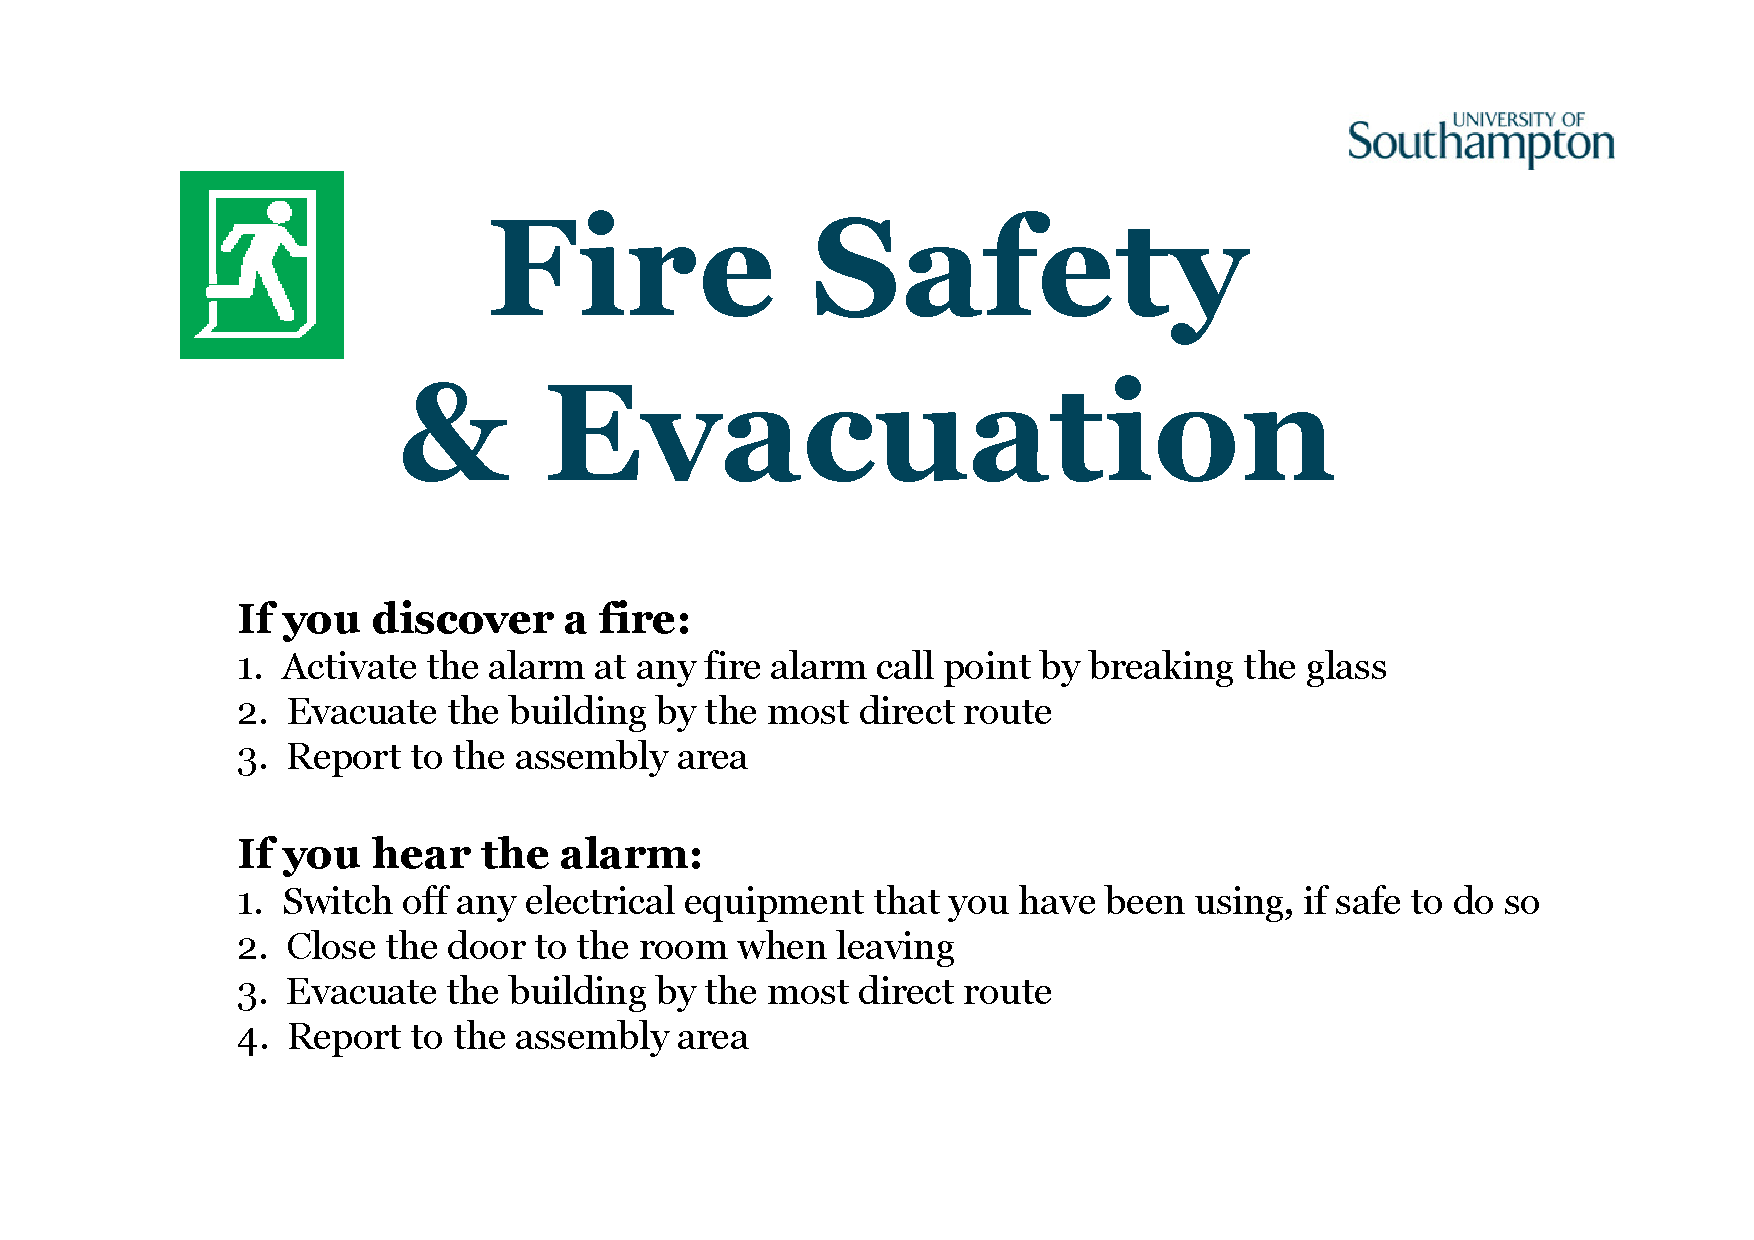
\includepdf[scale=1.0,landscape]{extras/Fire1.pdf}

\end{document}

